\section{Технологический раздел} \label{tech}

В данном разделе выбраны и обоснованы средства реализации, работана база данных, а также будет разработан интерфецс доступа к данным. Выполнено покрытие тестами публичного API приложение, протестирован триггер.

\subsubsection{Резальтат выбора объектной базы данных}

Для реализации проекта среди 2 рассмотренных вариантов была выбрана база данных Yandex S3, так как она доступна в России и удовлетворяет всем требованиям.


\subsubsection{Результат выбора реляционной базы данных}

В качестве основной базы данных принято использовать PostgreSQL, так как она удовлетворяет заданным требованиям и, кроме того, выбранный для разработки фреймворк userver имеет лучшую поддержку именно этой базы данных.

\subsection{Сущности объектной базы данных}

Единственная сущность объектной базы данных --- бинарный файл. Доступ к нему осуществляется по имени файла. Имя файла --- его идентификатор (полу в таблице file{\_}meta).

Проектирование ролевой модели для объектной базы данных разрабатываемого приложения нецелесообрвзно.

\subsection{Сущности реляционной базы данных}

Ниже представлены разработанные сущности базы данных.

\subsubsection{Таблицы}

На рисунке \ref{fig:dr-er} представлены сущности-таблицы полученной базы данных. Для обеспечения целостности данных используются внешние ключи, ограничения на уникальность первичного ключа.

\begin{figure}[h!]
	\centering{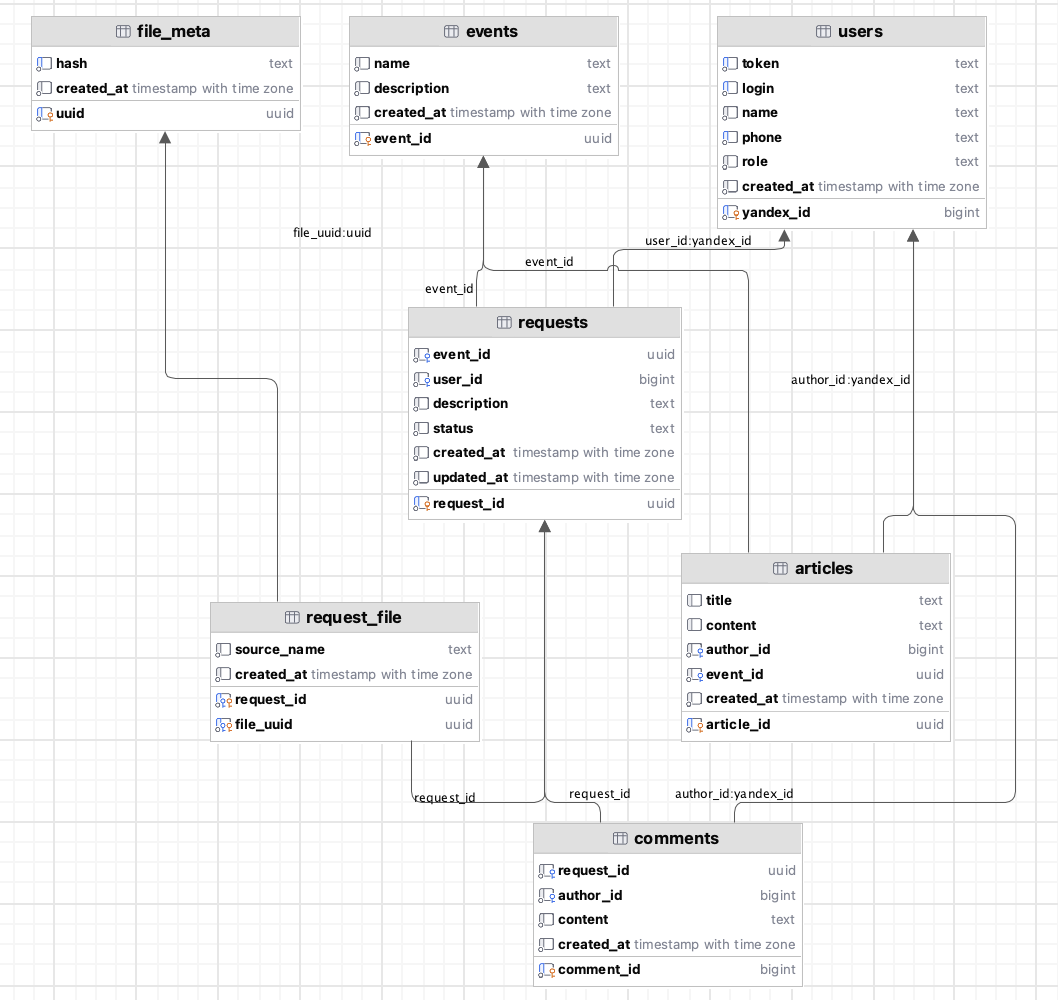
\includegraphics[scale=0.5]{img/db-er.png}}
	\caption{ER-диаграмма базы данных}
	\label{fig:dr-er}
\end{figure}

\subsubsection{Индекс}

В таблице requests используется стандартный b-tree индекс на поле user{\_}id. Использование необходимо обеспечения быстродействия запроса из листинга \ref{lst:exec_time} и для проведения исследования.


\subsubsection{Триггер}

На рисунке \ref{fig:trigger} представлена диаграмма спроектированного триггера.

\begin{figure}[h!]
	\centering{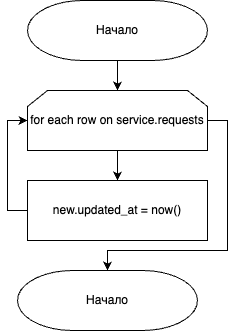
\includegraphics[scale=0.8]{img/trigger.png}}
	\caption{Блок-схема триггера}
	\label{fig:trigger}
\end{figure}

Триггер гарантирует корректность метки времени updated{\_}at таблицы requests. Для тестирования триггера написаны функциональные тесты на языке Python c использованием библиотеки pytest. В таблице \ref{tab:trigger_tests} приведены сценарии тестирования.

\begin{table}[ht!]
	\centering
	\caption{\label{tab:trigger_tests} Сценарии тестирования триггера}
	\begin{tabular}{|l|l|l|l|l|}
		\hline
		\textbf{Событие} & \textbf{Ожидаемый результат} & \textbf{Рельный результат}\\
		\hline
		Изменилось поле description & updated{\_}at = now() & updated{\_}at = now() \\
		\hline
		Изменилось поле status & updated{\_}at = now() & updated{\_}at =  now() \\
		\hline
		Попытка изменить updated{\_}at & updated{\_}at = now() & updated{\_}at =now() \\
\hline
		
	\end{tabular}
\end{table}

\subsubsection{Роли}

Помимо ролевой модели на уровне приложения разработана для дополнительных гарантий безопасности дополнительно разраотана ролевая модель на уровне приложения.  Права пользователей представлены в таблице \ref{tab:roles}.

\begin{table}[ht!]
	\centering
	\caption{\label{tab:roles} Ролевая модель на уровне базы данных}
	\begin{tabular}{|l|l|l|l|l|}
		\hline
		\textbf{Действие} & \textbf{Таблица} & \textbf{everybody} & \textbf{modarator} &  \textbf{admin}\\
		\hline
		select & все таблицы & да & да & да \\
		\hline
		insert, update & requests & да & да & да \\
		\hline
		insert, update, delete & events & нет & да & да \\
		\hline
		insert, update & users & да & да & да \\
		\hline
		insert, update, & requests{\_}file{\_}meta & да & да & да \\
		\hline
		insert, update & file{\_}meta & да & да & да \\
		\hline
		insert, update, delete & permisisions & нет & нет & да \\
		\hline
		insert, update & comments & да & да & да \\
		\hline

	\end{tabular}
\end{table}

Такая ролевая модель на уровне базы данных обеспечит пользователей минимальными необходимыми правами для доступа к просмотру и модификации данных.

\subsection{Обеспечение целостности данных}

Для обечспечения целостности предприняты следующие меры:
\begin{enumerate}
	\item добавлены внешние ключи (полный список можно увидеть на er-диаграмме на рисунке \ref{fig:dr-er});
	\item доавлено ограничение на уникальность хеша файла, это позволит гарантировать отсутсвие в системе двух одинаковых файлов;
	\item создан и протестирован триггер на поле updated{\_}at таблицы requests.
\end{enumerate}


\subsection{Интерфейс доступа к данным}

Доступ к данным осуществляется методом отправки http запроса на сервер, на котором развернуто приложение. Ниже приведено опсание эндпоинтов.

\begin{enumerate}
	\item /v1/request GET --- получение информации о запросе по его идентификатору. 
	\item /v1/requests GET --- получение информации о всех запросах, доступных для просмотра.
	\item /v1/requests POST --- создание/обновление запроса.
	\item /v1/request/status PATCH --- обновление статуса заявки.
	\item /v1/request/comment POST --- добавление комментария к заявке.
	\item /v1/file GET --- получение файла по его идентификтору.
	\item /v1/file POST --- добавление файла (приложения).
	\item /v1/events GET --- просмотр списка мероприятий.
	\item /v1/event POST --- создание мероприятия.
	\item /v1/event DELETE --- удаление мероприятия.
\end{enumerate}

\subsection{Вывод}

Разработаны и протестированы сущности базы данных, разработан интерфейс взаимодействия с данными.

\pagebreak